\documentclass[tikz,border=6pt]{standalone}
\usetikzlibrary{calc,intersections}

\begin{document}
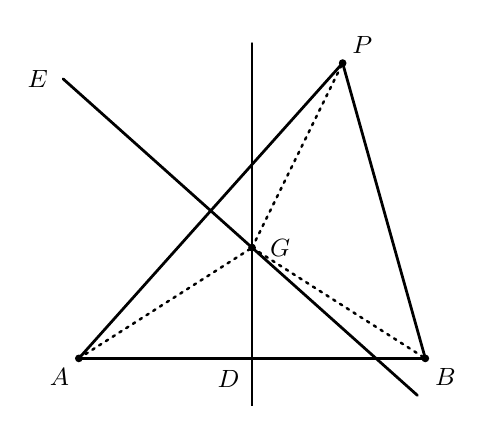
\begin{tikzpicture}[font=\small,line cap=round,line join=round]
\clip (-2.85,-0.6) rectangle (2.6,4.2);
% ----- given points -----
\coordinate (A) at (-2.2,0);
\coordinate (B) at ( 2.2,0);
\coordinate (P) at ( 1.15,3.75);

% midpoint D of AB
\coordinate (D) at ($(A)!0.5!(B)$);

% midpoint M of AP
\coordinate (M) at ($(A)!0.5!(P)$);

% direction perpendicular to AP:
% if v = P-A = (vx,vy) then v_perp = (-vy, vx)
\path let \p1=($(P)-(A)$) in
  coordinate (Mp1) at ($(M)+(-.35*\y1,.35*\x1)$)
  coordinate (Mp2) at ($(M)-(-.25*\y1,.25*\x1)$);

% ----- define the two perpendicular bisectors as paths and intersect them -----
\path[name path=bisAB] ($(D)+(0,-3.0)$) -- ($(D)+(0,5.0)$);
\path[name path=bisAP] ($(Mp2)!3!(M)$) -- ($(Mp1)!3!(M)$);

% intersection point G of the two bisectors
\path[name intersections={of=bisAB and bisAP, by=G}];

% choose a visible point E on bisAP (to the left of G, like the scan)
\coordinate (E) at ($(G)!1!($(Mp2)!3!(M)$)$);

% ----- draw main triangle APB -----
\draw[line width=1.0pt] (A) -- (B);
\draw[line width=1.0pt] (A) -- (P);
\draw[line width=1.0pt] (B) -- (P);

% ----- draw the bisectors (solid) -----
\draw[line width=1.0pt] ($(D)+(0,-1.1)$) -- ($(D)+(0,4.0)$); % GD
\draw[line width=1.0pt] ($(Mp2)!3!(M)$) -- ($(Mp1)!3!(M)$);  % GE (perp bisector of AP)

% ----- dotted auxiliary segments (as in the figure) -----
\draw[dotted, line width=0.9pt] (A) -- (G);
\draw[dotted, line width=0.9pt] (G) -- (P);
\draw[dotted, line width=0.9pt] (G) -- (B);

% ----- points + labels -----
\fill (A) circle (1.4pt) node[below left] {$A$};
\fill (B) circle (1.4pt) node[below right] {$B$};
\fill (P) circle (1.4pt) node[above right] {$P$};

\fill (G) circle (1.4pt) node[right=3pt] {$G$};

\node[below left=1pt] at (D) {$D$};
\node[left=2pt]  at (E) {$E$};

\end{tikzpicture}
\end{document}
